\documentclass[a4paper]{article}

\setlength{\oddsidemargin}{-1in}
\addtolength{\oddsidemargin}{0.05 \paperwidth}
\setlength{\evensidemargin}{-1in}
\addtolength{\evensidemargin}{0.05 \paperwidth}
\setlength{\textwidth}{0.9 \paperwidth}

\setlength{\topmargin}{-0.75in}
\addtolength{\topmargin}{0.05 \paperheight}
\setlength{\textheight}{\paperheight}
\setlength{\headheight}{0in}
\setlength{\headsep}{0in}
\setlength{\footskip}{0in}

\setlength{\parskip}{0.3cm}
\setlength{\parindent}{0pt}

\usepackage[T1]{fontenc}
\usepackage[utf8]{inputenc}
\usepackage[german]{babel}

\usepackage[default,scale=1.5]{opensans}
\usepackage[scaled=1.4]{beramono}
\linespread{1.7}

\usepackage{url}
\usepackage{graphicx}

\usepackage{grid-system}

\usepackage{color}
\definecolor{freifunkpink}{RGB}{215,0,73}
\definecolor{freifunkyellow}{RGB}{255,191,0}
\definecolor{lightgrey}{RGB}{220,220,220}

\usepackage{enumitem}
\setlist[itemize]{leftmargin=*}

\begin{document}
\thispagestyle{empty}

\begin{center}
\Huge \textit{\textbf{\textcolor{freifunkpink}{Freifunk Darmstadt}}} \\
\vspace{0.6cm}
\large
Freifunk ist ein regionales WLAN-Netz in Nutzerhand.\\
Mach mit! Erweitere das Netz in Deiner Nachbarschaft\\
indem Du selbst einen Freifunk-fähigen Router aufstellst.\\
\normalsize

\vspace{1.7cm}

\hspace*{-0.05 \paperwidth}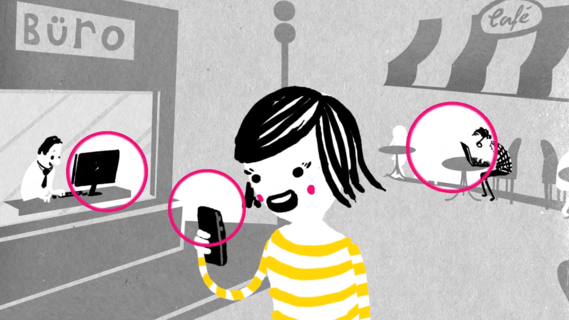
\includegraphics[width=\paperwidth]{../images/city_center}
\end{center}

\vspace{0.8cm}

\begin{Row}
    \begin{Cell}{5}
      \textbf{Was kann man damit tun?} \\
      Durch Freifunk werden z.B. ein lizenzfreies Community-Radio, die Übertragung
      lokaler Events und die gemeinsame Nutzung eines Internetanschlusses möglich.
      Auch bietet das Netz die Möglichkeit, ganz praxisnah einmal hinter die
      Kulissen moderner Netzwerktechnologie zu schauen.
    \end{Cell}
    \begin{Cell}{4}
      \textbf{Wir verstehen frei als:} \vspace*{-0.18cm}
	    \begin{itemize}
        \item[\textcolor{freifunkpink}{\Large$\bullet$}] öffentlich \vspace*{-0.3cm}
        \item[\textcolor{freifunkpink}{\Large$\bullet$}] anonym zugänglich \vspace*{-0.3cm}
        \item[\textcolor{freifunkpink}{\Large$\bullet$}] nicht kommerziell \vspace*{-0.3cm}
        \item[\textcolor{freifunkpink}{\Large$\bullet$}] unzensiert \vspace*{-0.3cm}
        \item[\textcolor{freifunkpink}{\Large$\bullet$}] gemeinschaftlich betrieben\vspace*{-0.3cm}
        \item[\textcolor{freifunkpink}{\Large$\bullet$}] unabhängig\vspace*{-0.3cm}
        \item[\textcolor{freifunkpink}{\Large$\bullet$}] dezentral organisiert
    	\end{itemize}
    \end{Cell}
\end{Row}

\newpage
\thispagestyle{empty}

\begin{Row}
  \begin{Cell}{5}
    \textbf{Werde ein Teil von Freifunk} \\
    Freifunk-Netze sind Selbstmach-Netze. Auch Du kannst dazu beitragen, indem Du
    einen Router mit der Freifunk-Software aufstellst und Deinen Internetzugang
    mit anderen teilst. Wenn viele mitmachen, entsteht ein flächendeckendes,
    freies WLAN-Netz.
  \end{Cell}
  \begin{Cell}{5}
    \textbf{Wer funkt, muss hoch hinaus!}\\
    Zum Aufbau eines unabhängigen und krisensicheren Netzes sind wir auf höher
    gelegene Standorte zum Aufbau von Richtfunkstrecken angewiesen. Solltest Du
    Zugang zu einem höheren Gebäude und Interesse an Freifunk haben, würden wir
    uns freuen, von Dir zu hören.
  \end{Cell}
\end{Row}

\vspace{1.5em}

\begin{Row}
  \begin{Cell}{5}
    \textbf{Unsere Ziele}\vspace*{-0.35cm}
		\begin{itemize}
			\setlength{\itemindent}{0.5em}
			\item[\textcolor{freifunkpink}{\Large$\bullet$}] Aufklärung und Sensibilisierung zum Thema Kommunikationsfreiheit\vspace*{-0.3cm}
			\item[\textcolor{freifunkpink}{\Large$\bullet$}] Verminderung der digitalen Spaltung\vspace*{-0.3cm}
			\item[\textcolor{freifunkpink}{\Large$\bullet$}] Ungehinderte Verbreitung von Wissen und Ressourcen\vspace*{-0.3cm}
			\item[\textcolor{freifunkpink}{\Large$\bullet$}] Menschen dazu befähigen, eigene Netze aufzubauen und zu betreiben\vspace*{-0.3cm}
			\item[\textcolor{freifunkpink}{\Large$\bullet$}] Vorhandene und neue Sozialstrukturen fördern und vernetzen\vspace*{-0.3cm}
		\end{itemize}
  \end{Cell}
\end{Row}


\begin{center}
	\vspace{.3cm}
	\hspace*{-0.05 \paperwidth}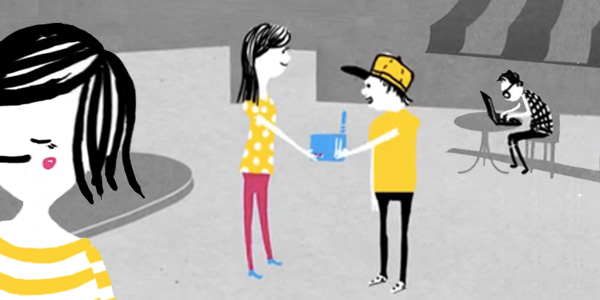
\includegraphics[width=\paperwidth]{../images/community_router}
\end{center}

Weitere Informationen findest Du auf \textbf{https://darmstadt.freifunk.net}.\\
Per Mail erreichst Du uns unter \textbf{info@darmstadt.freifunk.net}.

Wenn Du beim Aufbau des freien Netzes mitmachen möchtest, dann schau doch einfach
mal bei unserem wöchentlichen \textbf{offenen Treffen} vorbei. Du bist herzlich eingeladen!

\end{document}
